\begin{frame}
    \frametitle{Varying input: MMR build share}
    \begin{columns}
        \column{4.5cm}
            \begin{itemize}
                \item All of the metrics increase as build share increases
                \item \gls{SNF} mass has the smallest increase in 
                      relative change
                \item \gls{HALEU} \gls{SWU} capacity has the largest relative increase 
                \item These results are primarily because of the deployment scheme    
            \end{itemize}
        \column{5.5cm}
            \begin{figure}
                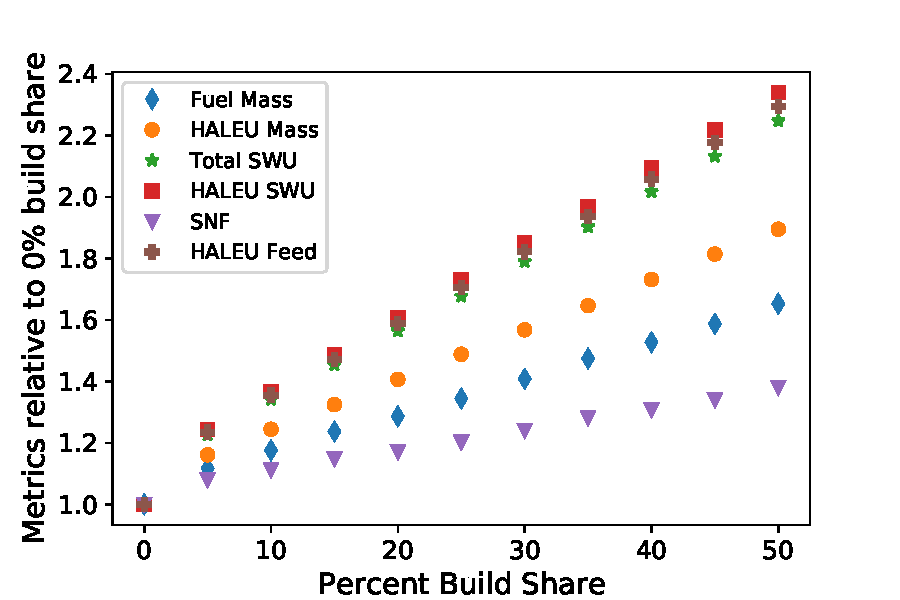
\includegraphics[scale=0.45]{mmr.pdf}
                \caption{Relative change in metrics as a function MMR 
                build share.}
                \label{fig:mmr}
            \end{figure}

\end{columns}
\end{frame}

\begin{frame}
    \frametitle{Varying MMR build share -- Number of reactors deployed}
    \begin{figure}
        \centering
        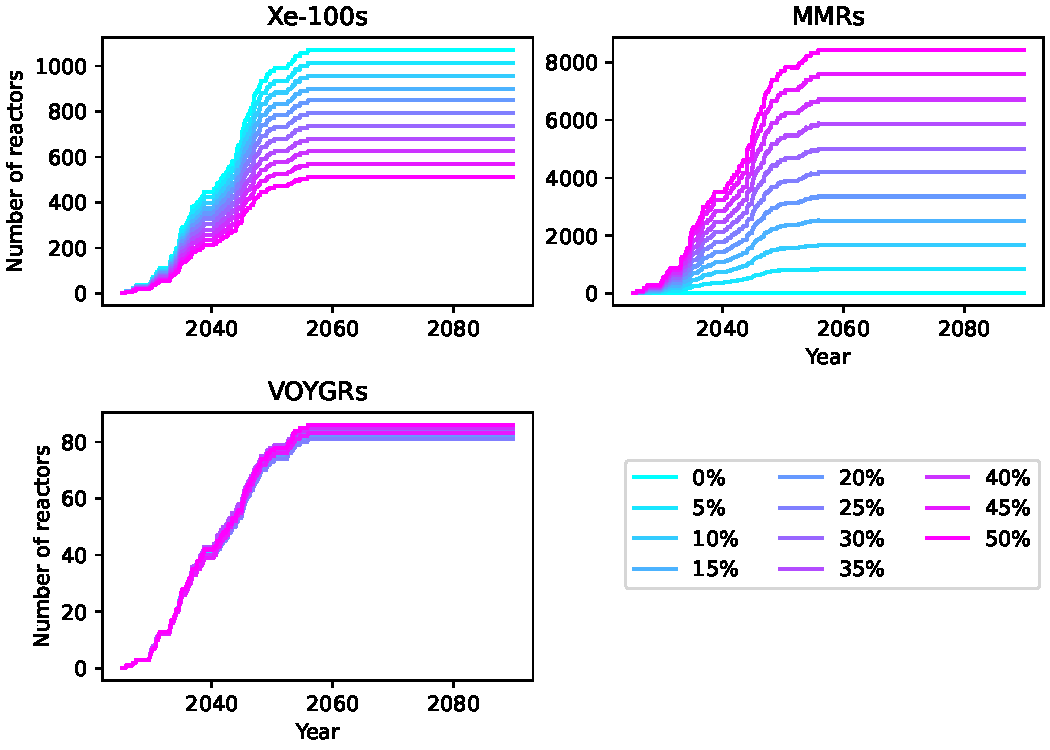
\includegraphics[scale=0.6]{mmr_combined_reactors.pdf}
        \caption{Number of MMRs deployed as a function of time when the 
        MMR build share is varied.}
    \end{figure}
\end{frame}
\begin{frame}
    \frametitle{Varying input: Xe-100 build share}
    \begin{columns}
        \column{4.5cm}
            \begin{itemize}
                \item The \gls{HALEU}-related metrics increase
                      with increasing build share
                \item Total \gls{SNF} and total fuel mass decrease with 
                      increasing build share
                \item Total \gls{SWU} capacity is relatively constant, at most 
                      a relative change of 1.06
            \end{itemize}
        \column{5.5cm}
            \begin{figure}
                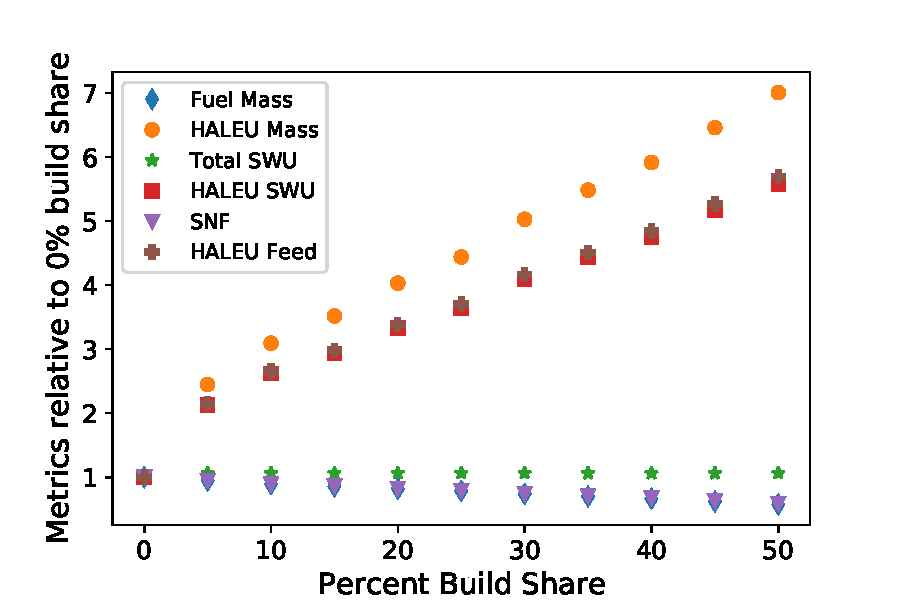
\includegraphics[scale=0.45]{xe100.pdf}
                \caption{Relative change in metrics as a function of Xe-100 
                build share \protect\cite{bachmann_sensitivity_2022}.}
                \label{fig:xe100}
            \end{figure}

\end{columns}
\end{frame}
   

\begin{frame}
    \frametitle{Varying input: VOYGR build share}
    \begin{columns}
        \column{4.5cm}
            \begin{itemize}
                \item Fuel mass and SNF mass increase while \gls{HALEU}
                      metrics decrease 
                \item Total SWU capacity is relatively constant
                \item Opposite trends as increasing Xe-100 build share
                \item As the build share increases, the number of Xe-100s
                      decreases and the number of MMRs is fairly constant
                
            \end{itemize}
        \column{5.5cm}
        \begin{figure}
            \centering 
            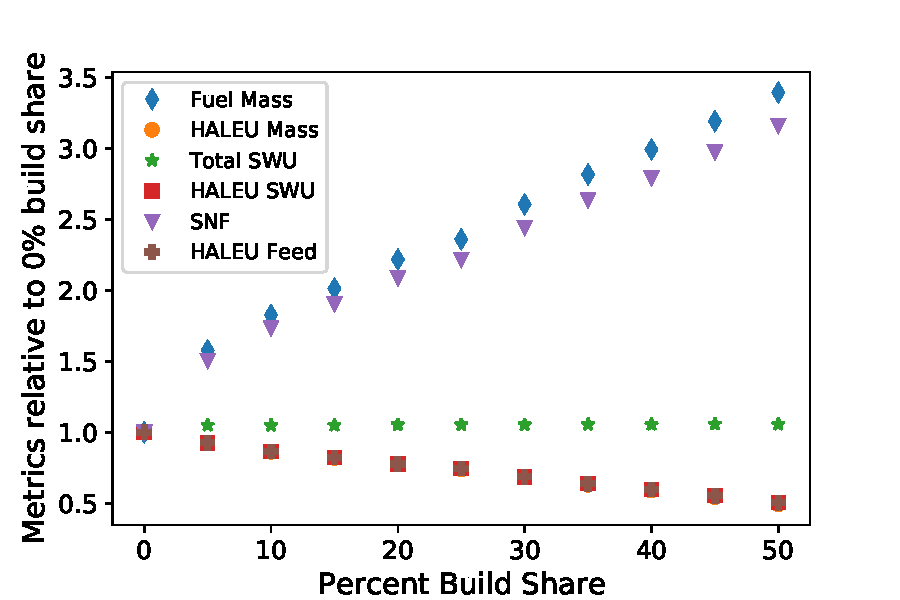
\includegraphics[scale=0.45]{voygr.pdf}
            \caption{Relative change in metrics as a function 
            of VOYGR build share \protect\cite{bachmann_sensitivity_2022}.}
            \label{fig:voygr}
        \end{figure}
    \end{columns}
\end{frame}